\documentclass[a4paper, 11pt, final, garamond]{book}
\usepackage{cours-preambule}

\raggedbottom

\makeatletter
\renewcommand{\@chapapp}{Travaux pratiques -- TP}
\makeatother

\let\SavedIndent\indent
\protected\def\indent{%
  \begingroup
    \parindent=\the\parindent
    \SavedIndent
  \endgroup
}
\setlength{\parindent}{0pt}

\begin{document}
\setcounter{chapter}{4}

\chapter{Circuits en r\'egime permanent}

\section{Objectifs}

\begin{itemize}
    \item Réaliser des montages électriques lisibles~;
    \item Mesurer une tension et une intensité directement à l’aide d’un
        multimètre numérique.
    \item Mesurer une résistance interne de manière indirecte avec un pont
        diviseur de tension.
    \item Réaliser une régression linéaire.
\end{itemize}

\section{S'approprier}
\subsection{Le multimètre}

\begin{wrapfigure}[20]{R}{.3\linewidth}
    \vspace*{-20pt}
    \centering
    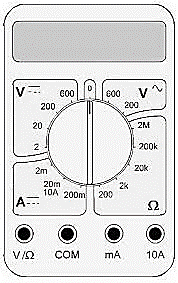
\includegraphics[width=\linewidth]{multi}
\end{wrapfigure}
Un multimètre permet de mesurer une intensité (ampèremètre), une différence de
potentiel (voltmètre) ou une résistance (ohmmètre). Il est nécessaire de :
\begin{itemize}
    \item Brancher l’appareil en utilisant les bonnes bornes (la borne COM est
        toujours utilisée).
    \item Choisir le bon mode (AC ou DC).
    \item Choisir le bon calibre.
\end{itemize}

\centers{\fbox{Les modes AC et DC}}

Le mode DC (courant continu, Direct Current), de symbole

\includegraphics[height=12pt]{dc}, permet de mesurer la valeur moyenne d’une
tension ou d’une intensité~: 

\begin{equation*}
    \left\langle s \right\rangle = \frac{1}{T} \int_{t_0}^{t_0+T} s(t) \dt
\end{equation*}

Le mode AC (courant alternatif, Alternating Current), de symbole

\includegraphics[height=12pt]{ac}, permet de mesurer la valeur efficace d’une
tension ou d’une intensité~:

\begin{equation*}
    S_{\rm eff} = \sqrt{ \left\langle s^2 \right\rangle} = \sqrt{\frac{1}{T}
    \int_{t_0}^{t_0+T} s^2(t) \dt}
\end{equation*}

\centers{\fbox{Choix de calibre}}

Il faut prendre le plus petit calibre au-dessus de la valeur mesurée pour
maximiser la précision de la mesure.

\subsection{Gestion de la masse d'un circuit}

Dans un circuit électrique, il ne peut y avoir qu’un seul point de référence des
potentiels (masse), donc il ne peut donc y avoir qu’une seule masse dans le
circuit (sauf si on utilise un transformateur d’isolement, voir le prochain TP).
Une bonne habitude consiste à utiliser des câbles noirs uniquement pour indiquer
où se trouvent les masses du circuit. Tous les câbles noirs d’un circuit doivent
alors être reliés entre eux~!

\begin{itemize}
    \item Un fil NOIR est toujours à la masse du circuit.
    \item Un fil NOIR se branche uniquement sur un fil NOIR.
\end{itemize}

\section{Réaliser et valider}
\subsection{Matériel}
\leftcentersright{Matériel sur votre paillasse~:}{}{ Matériel sur le bureau de
læ professeurx~:}

\begin{minipage}{0.49\linewidth}
    \begin{itemize}
        \item Une alimentation stabilisée.
        \item Un générateur basses fréquences.
        \item Une boîte de résistances variables (boite à décades).
        \item 2 multimètres (un Métrix et un du type de celui schématisé
            ci-dessus, portable).
        \item Plaquette de branchement et fils.
    \end{itemize}
\end{minipage}
\hfill
\begin{minipage}{0.49\linewidth}
    \begin{itemize}
        \item Résistances de différentes valeurs : (\SI{1}{k\ohm},
            \SI{2.2}{k\ohm}, \SI{10}{k\ohm}, \SI{5}{M\ohm} et \SI{10}{M\ohm}).
    \end{itemize}
\end{minipage}

\subsection{Les lois de base des circuits électriques}
\subsubsection{La loi d'Ohm}
\begin{wrapfigure}[5]{R}{.3\linewidth}
    %\vspace*{-20pt}
    \centering
    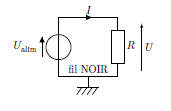
\includegraphics[width=\linewidth]{lohm}
\end{wrapfigure}
~\vspace{-20pt}
\begin{itemize}
    \item Réaliser le montage ci-contre avec une résistance $R$ de
        \SI{10}{k\ohm}.
    \item Le générateur à utiliser est l’alimentation stabilisée variable (côté
        tension variable). La mettre sur \SI{5}{V} environ.
    \item Vérifier la loi d’Ohm à l’aide d’une mesure de $U$ (grâce au voltmètre
        «~portable~») et de $I$ (grâce au multimètre Métrix).
    \item ATTENTION aux branchements des multimètres !! 
\end{itemize}

\subsubsection{Lois des mailles et des nœuds}
\begin{wrapfigure}[5]{R}{.4\linewidth}
    %\vspace*{-20pt}
    \centering
    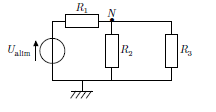
\includegraphics[width=\linewidth]{ldmn}
\end{wrapfigure}
~\vspace{-20pt}
\begin{itemize}
    \item Réaliser le montage ci-contre en utilisant de nouveau l’alimentation
        stabilisée variable et en donnant aux trois résistances des valeurs
        différentes comprises par exemple entre \SI{1}{k\ohm} et \SI{10}{k\ohm}.
    \item Vérifier expérimentalement la loi des mailles sur la maille de gauche
        en utilisant les multimètres.
    \item Vérifier aussi la loi des nœuds en N à l’aide des multimètres (vous
        pourrez emprunter un 3\ieme multimètre à un de vos voisins).
\end{itemize}

\subsubsection{Pont diviseur de tension}
\begin{wrapfigure}[5]{R}{.2\linewidth}
    %\vspace*{-20pt}
    \centering
    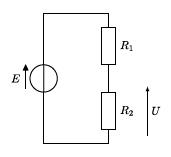
\includegraphics[width=\linewidth]{pontdiv}
\end{wrapfigure}

On réalise le montage ci-contre, dans lequel $E = \SI{5}{V}$, $R_2 =
\SI{1}{k\ohm}$ et $R_1$ est une résistance variable. Les résistances $R_1$ et
$R_2$ étant en série, le pont diviseur de tension conduit à : $\DS U =
\frac{R_2}{R_1+R_2}E$.

\begin{itemize}
    \item Mesurer plusieurs valeurs de la tension $U$ pour plusieurs valeurs de
        la résistance $R_1$ (entre \num{0.1} et \SI{10}{k\ohm}).
    \item Pour chaque mesure, calculer $\DS \frac{R_2}{R_1+R_2} \frac{E}{U}$.
    \item À l’aide d’un calcul d’erreur relative, conclure si la formule du pont
        diviseur est compatible avec les valeurs de $\DS \frac{R_2}{R_1+R_2}
        \frac{E}{U}$.
\end{itemize}

\subsection{Résistances d'entrée et de sortie d'un dipôle}
\subsubsection{Résistance de sortie du GBF}

Dans cette partie, on utilise le générateur basse fréquence (GBF) en mode
continu (DC pour direct current) en \textbf{tirant le bouton offset} et le
tournant de façon à lui faire délivrer \SI{5}{V} environ. Il ne faut, par
ailleurs, qu’aucun des boutons de la ligne du haut ne soit enfoncé. On utilisera
la sortie \SI{50}{\ohm} (aussi notée \textit{output}).\bigbreak

\begin{wrapfigure}[11]{R}{.45\linewidth}
    %\vspace*{-20pt}
    \centering
    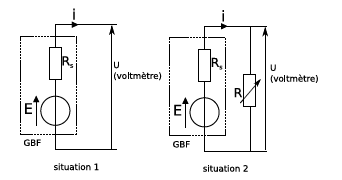
\includegraphics[width=\linewidth]{gbf}
\end{wrapfigure}
Le GBF n’est pas une source idéale de tension~: c’est une source de tension que
l’on peut modéliser par un générateur de Thévenin caractérisé par une
\textit{fem} $E$ et une résistance de sortie $R_s$, comme dans la situation 1.

Dans la situation 2, $R$ est une résistance variable (boite à décades).
\begin{enumerate}
    \item Exprimer $U$ en fonction de $E$ dans la situation 1. En déduire un
        protocole de mesure de $E$.
    \item Exprimer $U$ en fonction de $E$, $R$ (résistance variable) et $R_s$
        dans la situation 2. Dans le cas particulier où $U=E/2$, quelle est la
        relation entre  $R$ et $R_s$~? En déduire un protocole de mesure de
        $R_s$.
\end{enumerate}

\subsubsection{Résistance d'entrée d'un voltmètre}

\begin{wrapfigure}[6]{R}{.3\linewidth}
    \vspace*{-35pt}
    \centering
    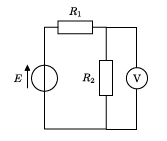
\includegraphics[width=\linewidth]{voltreel}
\end{wrapfigure}
~\vspace{-20pt}
\begin{itemize}
    \item Un voltmètre idéal est supposé de résistance infinie. Ainsi, branché
        en dérivation, il ne perturbe pas le système en absorbant une partie du
        courant. En réalité, un voltmètre possède une résistance interne grande
        mais finie, appelée résistance d’entrée du Voltmètre.
    \item Avec un GBF générant une tension continue, réaliser le montage
        ci-contre avec $R_1 \approx \SI{5}{M\ohm}$ et $R_2 \approx
        \SI{10}{M\ohm}$.
        \begin{enumerate}
            \item Quelle devrait être la valeur mesurée par le voltmètre, si
                celui-ci était idéal ?
            \item Faire la mesure. Que pensez-vous de ce résultat ? Pouvez-vous
                donner une explication ?
        \end{enumerate}
\end{itemize}

\encadre{Conclure}

\end{document}
